\documentclass[a4paper]{article}

% font stuff
\usepackage{fouriernc}
\usepackage[T1]{fontenc}

\usepackage{amsmath}
\usepackage{amssymb}
\usepackage{amsthm}
\usepackage[retainorgcmds]{IEEEtrantools}
\usepackage{enumitem} % no space between enum lists

\usepackage{tikz}
\usetikzlibrary{positioning}
\usetikzlibrary{matrix}


\newcommand{\below}{\sqsubseteq}
\newcommand{\arr}{\rightarrow}
\newcommand{\todo}[1]{\smallskip \noindent \emph{todo: #1} \smallskip}
%\newcommand{\todo}[1]{}
\newcommand{\semantics}[1]{\llbracket #1 \rrbracket}
\newcommand{\lub}{\bigsqcup}
\newcommand{\set}[1]{\{\,#1\,\}}
% partial function arrow
% https://tex.stackexchange.com/questions/47142/how-to-tex-an-arrow-with-vertical-stroke
\newcommand{\pfun}{\mathrel{\ooalign{\hfil$\mapstochar\mkern5mu$\hfil\cr$\to$\cr}}}
\newcommand{\isdefined}{\!\downarrow}

\newcommand{\bbN}{\mathbb{N}}
\newcommand{\bbC}{\mathbb{C}}
\newcommand{\bbD}{\mathbb{D}}
\newcommand{\bbE}{\mathbb{E}}

\newcommand{\aand}{\ \wedge \ }
\newcommand{\oor}{\ \vee \ }

\newcommand{\product}{\!\times\!}


% They all use the same counter, reset at section boundaries
% This gives a running number:
% Section 1
%   Theorem 1.1
%   Definition 1.2
%   Lemma 1.3
% Section 2
%   Definition 2.1
%   Lemma 2.2
%   ...
\newtheorem{definition}{Definition}[section]
\newtheorem{theorem}[definition]{Theorem}
\newtheorem{proposition}[definition]{Proposition}
\newtheorem{lemma}[definition]{Lemma}
\newtheorem{corollary}[definition]{Corollary}

\begin{document}

\title{Thesis}
\author{Markus Klinik}
\maketitle

\begin{abstract}

Abstract

\end{abstract}

\section{Introduction}

Introduction

\todo{fix location of qed signs}

\section{Domain Theory}

\todo{The section on domains in \cite{Gunter1992} is based on his paper with
Scott from 1990}

\begin{definition}

Let $D$ be a poset, $S \subseteq D$. The \emph{least upper bound} (``lub'') of
$S$ is an element $x \in D$ such that:

\begin{equation} \label{eqnLub1}
\forall y \in S \ldotp y \below x
\end{equation}
\begin{equation} \label{eqnLub2}
\forall z \in D \ldotp (\forall y \in S \ldotp y \below z) \implies x \below z
\end{equation}

The lub of S, if it exists, is denoted interchangeably by
\begin{IEEEeqnarray*}{rCl}
\lub S = \lub_{x \in S} x = \lub \set{x \mid x \in S}
\end{IEEEeqnarray*}

\end{definition}


Line (\ref{eqnLub1}) states that the lub is above all elements: it is an upper
bound, and (\ref{eqnLub2}) states that the lub is below any other upper bound:
it is the least such. If a lub exists, it is unique. It is therefore justified
to call it \emph{the} lub.


\begin{definition}

A \emph{chain} $C$ in a poset is a linearly ordered subset, that is $\forall x,y
\in C \ldotp x \below y \oor y \below x$

\end{definition}


\begin{definition}

Let $D$ be a poset. A set $S \subseteq D$ is \emph{directed} iff every finite
$P \subseteq S$ has an upper bound in $S$.

\end{definition}


In literature on domain theory and semantics of programming languages, one
encounters three different definitions of complete partial orders.  There is
chain-completeness \cite{Moschovakis1994}, directed-completeness
\cite{DaveyPriestly1990}, \cite{Gunter1992}, and $\omega$-sequence-completeness
\cite{Allison1986}, \cite{Winskel1993}, \cite{BarrWells1990}. Abramsky and Jung
\cite{Abramsky1994} have a short discussion on the equivalence of these
definitions, but refer to further literature for proofs. The proof given here
occurs as an exercise in Davey and Priestly \cite{DaveyPriestly1990}.


\begin{definition} \label{defCpoDirectedComplete}

A directed-complete partial order, \emph{dcpo}, is a partial order where every
directed set has a least upper bound.

\end{definition}


\begin{definition} \label{defCpoChainComplete}

A chain-complete partial order, \emph{ccpo}, is a partial order where every chain
has a least upper bound.

\end{definition}


\begin{definition} \label{defCpoOmegaSequenceComplete}

An $\omega$-sequence-complete partial order, \emph{$\omega$-cpo}, is a partial
order where every non-decreasing sequence of elements $x_0 \below x_1 \below x_2
\below \ldots $ has a least upper bound.

\end{definition}


\begin{proposition} \label{propDefinitionsAreEquivalent}

These three definitions are equivalent.

\end{proposition}

For proposition \ref{propDefinitionsAreEquivalent} we give a round-robin proof,
of which two implications are fairly simple. The third implication is a bit more
involved, and requires the axiom of choice. We give a proof for the countable
case here because it is illustrative and it is the case we're interested in, and
refer to the literature for the uncountable case. \todo{refer to the literature}


\begin{proof}

$\ref{defCpoDirectedComplete} \implies \ref{defCpoChainComplete}$: Every chain
is a directed set.

$\ref{defCpoChainComplete} \implies \ref{defCpoOmegaSequenceComplete}$:
The image of a non-decreasing $\omega$-sequence is a chain.

$\ref{defCpoOmegaSequenceComplete} \implies \ref{defCpoDirectedComplete}$: Let
$D$ be an $\omega$-cpo as in definition
\ref{defCpoOmegaSequenceComplete}, let $S = \set{x_0, x_1, x_2, \ldots}
\subseteq D$ be countable and directed. For each finite $F \subseteq S$, let
$u(F)$ be an upper bound of $F$ in $S$.  Construct a sequence of sets $P_n
\subseteq S$ as follows,
\begin{IEEEeqnarray*}{rCl}
P_0 & = & \set{x_0} \\
P_{n+1} & = & P_n \cup \set{u(P_n \cup y_n), y_n}
\end{IEEEeqnarray*}

where $y_n$ is the $x_i \in S\backslash P_n$ with the smallest possible $i$.

Every $P_n$ is directed: $P_0$ certainly is, and any finite subset of $P_{n+1}$
has $u(P_n \cup y_n) \in P_{n+1}$ as upper bound.  As every $P_n$ is finite and
directed, taking its lub is justified.

Consider the $\omega$-sequence $Q$ = $\set{\lub P_n}_{n \in \bbN}$. For
all $n$, we have $P_n \subseteq P_{n+1}$ and thus $\lub P_n \below \lub
P_{n+1}$, so $Q$ is non-decreasing, and therefore has a lub $z$.  Each $x \in S$
eventually occurs in some $P_n$, and we have $x \below \lub P_n \below z$, so
$z$ is an upper bound of $S$. Any upper bound $z'$ of $S$ is also an upper bound
of $Q$, and therefore $z \below z'$, i.e. $z$ is the lub of $S$.

\end{proof}


The complication in the third implication comes from the fact that a directed
set doesn't need to be linearly ordered. Every directed set does however contain
a chain which threads through the whole set, eventually rising above all
elements. The lub of the chain is then the lub of the directed set.

This equivalence justifies simply talking about \emph{complete partial orders},
or \emph{cpos}. We use the definitions interchangeably, whichever is most handy
in a given situation.

The fixpoint theorem constructs least fixpoints using countable chains.
Even if a domain is uncountable, the chains for which we want lubs are therefore
at most countable. Whenever we consider chains, we mean countable ones.

A countable chain $\set{x_n \mid x \in \bbN}$ is always also a non-decreasing
sequence \begin{IEEEeqnarray*}{c} x_0 \below x_1 \below x_2 \below \ldots
\end{IEEEeqnarray*} and vice versa.

A sequence is \emph{eventually constant} iff there exists an $n \in \bbN$ such
that for all $m > n$, $x_n = x_m$.  An eventually constant non-decreasing
sequence is equivalent to a finite chain, and vice versa.

\subsection{The Category Cppo}


\begin{definition}

A cpo $D$ is \emph{pointed} iff it has a bottom element $\bot$ which satisfies
$\forall d \in D \ldotp \bot \below d$. Such a pointed cpo is called
\emph{cppo}.

\end{definition}

\begin{definition}

Let $C$, $D$ be partial orders. A function $f : C \arr D$ is \emph{monotone} iff
it is order preserving, that is for all $x, y \in C$,
\begin{IEEEeqnarray*}{rCl}
  x \below y \implies f(x) \below f(y)
\end{IEEEeqnarray*}

\end{definition}

\begin{definition}

Let $C$, $D$ be cpos. A function $f : C \arr D$ is \emph{continuous} iff it
is monotone and preserves lubs, that is for all chains $P \subseteq C$,
\begin{IEEEeqnarray*}{rCl}
  f(\lub_{x \in P} x) = \lub_{x \in P} f(x)
\end{IEEEeqnarray*}

\end{definition}

Note that if a function preserves lubs, it is monotone,
\begin{IEEEeqnarray*}{rCl}
  x \below y \implies
  y = \lub \set{x, y} \implies
  f(y) = f(\lub \set{x, y}) = \lub \set{f(x), f(y)} \implies
  f(x) \below f(y)
\end{IEEEeqnarray*}
but in a proof of continuity of a function $f$ we usually need to prove
monotonicity as a first step so that for a chain $P$, $\set{f(x) \mid x \in P}$
is again a chain. This motivates the explicit mention of
monotonicity in the definition of continuity.


\begin{lemma}

The identity function is continuous.

\end{lemma}

\begin{proof}

Let $P \in C$ be a chain. Then
\begin{equation*}
id(\lub P) = \lub P = \lub_{x \in P} id(x)
\end{equation*}

\end{proof}


\begin{lemma}

Composition of two continuous functions is continuous.

\end{lemma}

\begin{proof}

Let $f : C \arr D$, $g : D \arr E$ be continuous. Let $P \subseteq C$ be a
chain. Then
\begin{IEEEeqnarray*}{rCl}
(g \circ f)(\lub P) & = & g(f(\lub_{x \in P} x)) \\
  & = & g( \lub_{x \in P} f(x) ) \\
  & = & \lub_{x \in P} g(f(x)) \\
  & = & \lub_{x \in P} (g \circ f)(x)
\end{IEEEeqnarray*}

\end{proof}


\begin{corollary}

The complete pointed posets, together with continuous functions between them form
a category.  This category is called Cppo.

\end{corollary}


\begin{definition}

A category has the \emph{fixpoint property} iff for all objects $A$ and arrows
$f : A \arr A$ there exists an arrow $Y(f) : 1 \arr A$, the fixpoint of f, such
that $Y(f) = f \circ Y(f)$.

\begin{center}
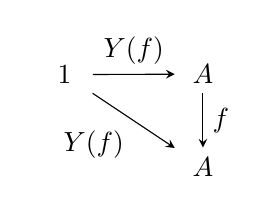
\begin{tikzpicture}
\matrix (m) [matrix of math nodes,row sep=2em,column sep=3em,minimum width=2em]
  {
     1 & A \\
     {} & A \\
  };
  \path[-stealth] (m-1-1) edge node [above] {$Y(f)$} (m-1-2);
  \path[-stealth] (m-1-1) edge node [below left] {$Y(f)$} (m-2-2);
  \path[-stealth] (m-1-2) edge node [right] {$f$} (m-2-2);
\end{tikzpicture}
\end{center}

\end{definition}


\begin{theorem} \label{thmFixpoint}

(Fixpoint Theorem) Cppo has the fixpoint property. In fact, every continuous
function on a cppo has a \emph{unique} least fixpoint.

\end{theorem}

\begin{proof}

Let $D$ be a cppo, $f : D \arr D$ a continuous function. We have to show that
there exists an element $x \in D$ such that $x = f(x)$. Consider the set
\begin{equation*}
F = \set{f^n(\bot) \mid n \in \bbN}.
\end{equation*}
This set is a chain, because for $n = 0$
we have $f^0(\bot) = \bot \below f(\bot)$. Now assume that $f^n(\bot) \below
f^{n+1}(\bot)$. Then $f(f^n(\bot)) \below f(f^{n+1}(\bot))$, so $f^{n+1}(\bot)
\below f^{n+2}(\bot)$. Because $F$ is a chain and $D$ a cppo, $F$ has a lub $x =
\lub F$.  We calculate:
\begin{IEEEeqnarray*}{rCl}
f(x) & = & f(\lub F) \\
     & = & \lub f(F) \IEEEyesnumber \label{lineFContinuous} \\
     & = & \lub \set{ f(f^n(\bot)) \mid n \in \bbN } \\
     & = & \lub \set{ f^{n+1}(\bot) \mid n \in \bbN } \\
     & = & \lub \set{ f^n(\bot) \mid n \in \bbN }
           \IEEEyesnumber \label{lineLubLeastElement} \\
     & = & \lub F = x
\end{IEEEeqnarray*}
Line (\ref{lineFContinuous}) is because $f$ is continuous, and line
(\ref{lineLubLeastElement}) is because omitting the least element in a chain
doesn't affect the lub.

To see that $x$ is the least fixpoint, let $y = f(y)$ be a fixpoint of $f$. We
have:
\begin{IEEEeqnarray*}{rCl}
\bot \below y & \implies & f(\bot) \below f(y) = y \\
 & \implies & \forall n \in \bbN \ldotp f^n(\bot) \below y \\
 & \implies & y \text{ is an upper bound of F} \\
 & \implies & \lub F = x \below y
\end{IEEEeqnarray*}

\end{proof}

This is the well-known fixpoint theorem, which is sometimes attributed to
Tarski, sometimes to Kleene, but while they both knew the result, its actual
origin seems to be lost in time \cite{Lassez1982}. The formulation given here
is due to Huwig \cite{Huwig1990}.


\begin{lemma} \label{lemCppoTerminalObject}
Cppo has a terminal object, the singleton $\set{\bot}$. \qed
\end{lemma}

\begin{lemma} \label{lemCppoBinaryProducts}
Cppo has binary products, defined pointwise as usual in algebra. \qed
\end{lemma}

\begin{lemma} \label{lemCppoExponentials}
Cppo has exponentials, that is
\begin{enumerate}[noitemsep]
  \item If $C$ and $D$ are cppos, then the space of continuous functions from
  $C$ to $D$, denoted $[C \arr D]$, forms a cppo.
  \item Currying and uncurrying are defined and are each others inverses. \qed
\end{enumerate}
\end{lemma}

\begin{corollary}
Cppo is cartesian closed.
\end{corollary}

A historical note on \ref{lemCppoExponentials}. Readers unfamiliar with domain
theory might be surprised that there exist domains $D$ which contain their own
function space $[D \arr D]$.  This result is due to Scott [TODO], who set out to
prove this being impossible, while looking for a dentotational semantics of
the untyped lambda calculus. Intuitively, it is possible because the
requirement for functions in $[D \arr D]$ to be continuous restricts the
function space sufficiently as to not increase in cardinality.

So far, the situation in Cppo is quite satisfying. For a programming language
semantics however, we also want coproducts. Unfortunately, due to the following
results, the best we can hope for are approximations.  These results were known
before, but made precise by Huwig \cite{Huwig1990},

\begin{definition}
An \emph{initial object} in a category is an object $0$ such that for any object
A there exists a unique arrow $0_A : 0 \arr A$.
\end{definition}

The prototypical example for an initial object is the empty set in Set. But
there are categories where initial objects behave differently than the empty set
in Set, perhaps unintuitively so. Important examples are categories where
objects are algebraic structures whose signatures require the existence of
elements, like monoids and groups. There, the initial objects are not empty
sets. In such categories the equivalence $0 \cong 0 \product A$ may not hold.

\begin{lemma} \label{lem0xAisInitial}
In a CCC with initial object $0$ we have, for any object $A$, $0 \cong 0
\product A$.
\end{lemma}

\begin{proof}
It suffices to show that $0 \product A$ is initial. We know that the functor
$- \product A$ is left adjoint to the exponent functor $A \Rightarrow -$, and
left adjoints preserve colimits (\cite{MacLane71}, IV.6, V.5). The initial object is the colimit of the
empty diagram. Therefore, $0 \product A$ is initial as well.
\end{proof}

As concise as abstract proofs like this become, they aren't very illustrative.
The following alternative proof of \ref{lem0xAisInitial} is a bit longer, but
more insightful. The idea is that $0\product A$ is initial because all arrows $0
\product A \arr B$ are identical, and that is because their curried counterparts
are identical.

\begin{proof}
We show that $0 \product A$ is initial. Let $B$ be an object. Then the
arrow $f = 0_B \circ \pi_1\ :\ 0 \product A \arr B$ exists. To see that it is
unique, let $g : 0 \product A \arr B$ be an arrow. The exponent diagram of the
CCC gives us:
\begin{figure}[h]
\begin{center}
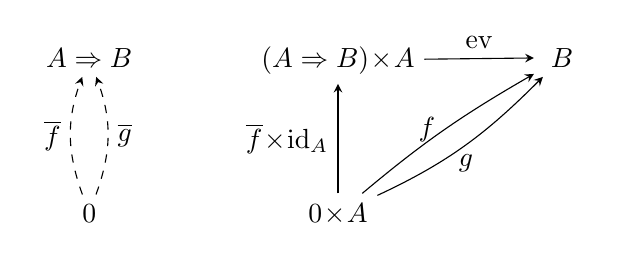
\begin{tikzpicture}
\matrix (m) [matrix of math nodes,row sep=4em,column sep=4em,minimum width=2em]
  {
     A \Rightarrow B & (A \Rightarrow B) \product A & B \\
     0 & 0 \product A \\
  };
  \path[-stealth, dashed] (m-2-1) [out=110,in=250] edge node [left] {$\overline{f}$} (m-1-1);
  \path[-stealth, dashed] (m-2-1) [out=70,in=290] edge node [right] {$\overline{g}$} (m-1-1);
  \path[-stealth] (m-1-2) edge node [above] {$\text{ev}$} (m-1-3)
    (m-2-2) edge node [left] {$\overline{f} \product \text{id}_A$} (m-1-2)
    (m-2-2) [out=40,in=210] edge node [left] {$f$} (m-1-3)
    (m-2-2) [out=25,in=225] edge node [below] {$g$} (m-1-3);
\end{tikzpicture}
\end{center}
\end{figure}

Where $\overline{f}$ is the curried counterpart of $f$. We have: $\overline{f} =
\overline{g}$, because $0$ is initial. Therefore $\overline{f}\product
\text{id}_A = \overline{g}\product \text{id}_A$, and
thus
\begin{IEEEeqnarray*}{c}
f\ =\ \text{ev} \circ \overline{f}\product\text{id}_A
 \ =\ \text{ev} \circ \overline{g}\product\text{id}_A
 \ =\ g.
\end{IEEEeqnarray*}

\end{proof}

\begin{lemma} \label{lem0isomorphic1}
In a category with fixpoints, initial and terminal objects are isomorphic.
\end{lemma}

\begin{proof}
As all endomorphisms have fixpoints, the identity on $0$ has a fixpoint
$Y(\text{id}_0) : 1 \arr 0$.  Composing it with the terminal map $!_0 : 0 \arr
1$ in both ways, the universal mapping properties of $0$ and $1$ give the
isomorphism $0 \cong 1$.
\end{proof}

\begin{definition}
A category is \emph{trivial} iff it has, up to isomorphism, exactly one object
with only the identity arrow.
\end{definition}

\begin{proposition} \label{propCCCNoFixpointInitialObject}
Any CCC with the fixpoint property and initial object is trivial.
\end{proposition}

\begin{proof}
Let $A$ be an object.  Then $1 \cong 0 \cong 0 \product A \cong 1 \product A
\cong A$. The first two equivalences are lemmas \ref{lem0xAisInitial} and
\ref{lem0isomorphic1}, the second holds because $- \product A$ is a functor, and
the last one always holds.
\end{proof}

\begin{proposition} \label{propCCCNoFixpointCoproducts}
Any CCC with the fixpoint property and binary coproducts is trivial.
\end{proposition}

\newcommand{\true}{\text{tt}}
\newcommand{\false}{\text{ff}}

\begin{definition}
A \emph{Boolean algebra} is an algebraic structure $(A, \wedge, \vee, \neg,
\true, \false)$ where $\wedge, \vee$ are binary operations, $\neg$ is a unary
operation, and $\true, \false$ are distinguished elements of $A$, such that the
Boolean algebra axioms hold.
\end{definition}

The definition of Boolean algebra can be lifted to category theory in the
obvious way. Operations and elements become arrows, and the Boolean algebra
axioms, which are all equations, become commutative diagrams.

\begin{definition}
A \emph{Boolean algebra object} in a CCC with coproducts is an object A,
together with arrows $\wedge, \vee : A \product A \arr A$, $\neg : A \arr A$,
$\true, \false : 1 \arr A$ such that the diagrams corresponding to the boolean
algebra axioms commute.
\end{definition}

\begin{lemma}
In a Boolean algebra $A$ where $\neg$ has a fixpoint $Y(\neg) = \neg Y(\neg)$,
all elements are identified.
\end{lemma}

\begin{proof}
\begin{IEEEeqnarray*}{rCl}
\true & = & Y(\neg) \oor \neg Y(\neg) \\
      & = & Y(\neg) \oor Y(\neg) \\
      & = & Y(\neg) \\
      & = & Y(\neg) \aand Y(\neg) \\
      & = & Y(\neg) \aand \neg Y(\neg) \\
      & = & \false
\end{IEEEeqnarray*}
Further, for any $a \in A$, $\false = a \wedge \false = a \wedge \true = a$.
\end{proof}

\begin{lemma}
In a CCC with coproducts, $2 = 1+1$ is a boolean algebra object. \qed
\end{lemma}

\begin{corollary}
In a CCC with fixpoints where the coproduct $1+1$ exists, the coproduct
injections $\true, \false : 1 \arr 1+1$ are identified.
\end{corollary}

\begin{proposition}
Every CCC with fixpoints where the coproduct $1+1$ exists is trivial.
\end{proposition}

\begin{proof}
We have that the functor $- \product A$ preserves coproducts, so $(1+1)\product
A = 2 \product A = A + A$ exists. From the embeddings $\true \product A, \false
\product A : 1 \product A \arr 2 \product A$, and the fact that $1 \product A
\cong A$ we get $\kappa_0 = \kappa_1 : A \arr A + A$. Consider the following
diagram.

\begin{center}
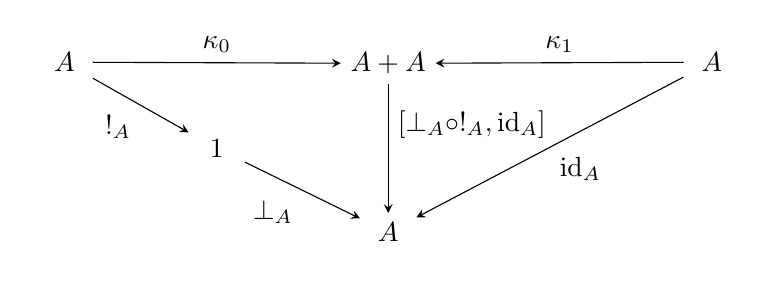
\begin{tikzpicture}
\matrix (m) [matrix of math nodes,row sep=1.7em,column sep=3.5em,minimum width=2em]
  {
     A & {} & A + A & {} & A \\
     {} & 1 \\
     {} & {} & A \\
  };
  \path[-stealth]
    (m-1-1) edge node [below left] {$!_A$} (m-2-2)
            edge node [above] {$\kappa_0$} (m-1-3)
    (m-1-3) edge node [above right] {$[\bot_A \circ !_A,\text{id}_A]$} (m-3-3)
    (m-1-5) edge node [above] {$\kappa_1$} (m-1-3)
            edge node [below right] {$\text{id}_A$} (m-3-3)
    (m-2-2) edge node [below left] {$\bot_A$} (m-3-3)
    ;
\end{tikzpicture}
\end{center}
The diagram commutes, and together with $\kappa_0 = \kappa_1$ we get $\bot_A
\circ !_A = \text{id}_A$. Furthermore, because $1$ is terminal, we have $!_A
\circ \bot_A = \text{id}_1$. We conclude that $A \cong 1$ for every $A$.
\end{proof}

\begin{proof}
(Proposition \ref{propCCCNoFixpointCoproducts}) In a CCC with binary coproducts,
$1+1$ exists.
\end{proof}

The singleton set $\set{\bot}$ is not initial in Cppo, because morphisms don't
preserve all cppo structure. Continuous functions must preserve lubs, but are
allowed to map $\bot$ to elements other that $\bot$. Otherwise the fixpoint
theorem would hold trivially, not giving rise to the application of fixpoint
semantics of recursive equations.

Propositions \ref{propCCCNoFixpointInitialObject} and
\ref{propCCCNoFixpointCoproducts} are due to Huwig \cite{Huwig1990}, and
demonstrate that if we want to use Cppo, or in fact any CCC with fixpoints,  as
model for programming languages, we won't get interpretations for sum types that
correspond to categorical coproducts. Nevertheless, we have a similar
construction that serves our purpose.

The disjoint union of cppos fails to have a bottom element, thus it is not a
cppo. There are two common ways to remedy this situation. We can either use a
construction that artificially adds a new bottom element below the disjoint
union, or one that identifies all bottom elements \cite{Gunter1992}. The former
is called \emph{separated sum}, the latter \emph{coalesced sum}.  Figure
\ref{figSeparatedAndCoalescedSum} sketches both these constructions of two given cppos.

\begin{figure}[ht]
\begin{center}

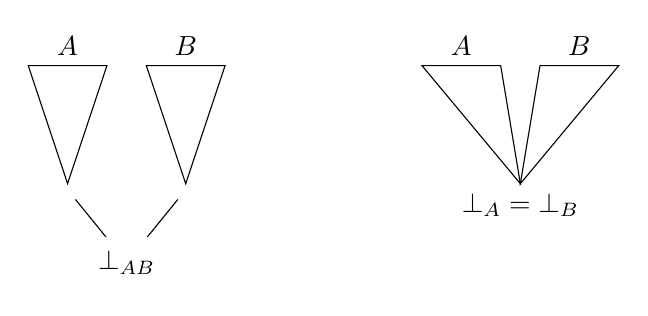
\begin{tikzpicture}[scale=1]
\draw (0,0) -- (0.5,0) node [above] {$A$} -- (1,0) -- (0.5,-1.5) -- cycle;
\begin{scope}[xshift=1.5cm]
\draw (0,0) -- (0.5,0) node [above] {$B$} -- (1,0) -- (0.5,-1.5) -- cycle;
\end{scope}
\draw[shape=rectangle] (0.6,-1.7) -- (1.25,-2.5)
  node [fill=white,inner sep=5pt] {$\bot_{AB}$} -- (1.9,-1.7)
;

\begin{scope}[xshift=5cm]
\draw (0,0) -- (0.5,0) node [above] {$A$} -- (1,0) -- (1.25,-1.5) -- cycle;
\begin{scope}[xshift=1.5cm]
\draw (0,0) -- (0.5,0) node [above] {$B$} -- (1,0) -- (-0.25,-1.5)
  node [below] {$\bot_A = \bot_B$}
  -- cycle;
\end{scope}
\end{scope}

\end{tikzpicture}

\end{center}
\caption{Separated and coalesced sum of two cppos.} \label{figSeparatedAndCoalescedSum}
\end{figure}

\begin{definition} \label{defCoalescedSum}
For objects $A$, $B$ in Cppo, define the \emph{coalesced sum} $A \oplus B$ as
the disjoint union of $A$ and $B$ where we identify the bottom elements.
\end{definition}

\begin{definition} \label{defSeparatedSum}
For objects $A$, $B$ in Cppo, define the \emph{separated sum} $A + B$ as $A
\dot\cup B \cup \bot_{AB}$ where $\bot_{AB} \not\in A \dot\cup B$ and $\bot_{AB}
\below \bot_A$ and $\bot_{AB} \below \bot_B$.
\end{definition}

It is not hard to see that both constructions yield cppos, and that the obvious
inclusions are continuous.

The coalesced sum is not useful for categorical fixpoint semantics of
programming languages. We intend to use a generalized fixpoint construction to
ensure existence of final coalgebras. The construction works by iterating a
functor on the terminal object. If we consider the functor $F(X) = 1 \oplus X$,
then the first iteration yields $F(1) = 1 \oplus 1 = 1$, so $F$ has a trivial
fixpoint. Using the separated sum however, this approach yields what we expect
to be the semantics for the lazy natural numbers.

As seen in \ref{propCCCNoFixpointCoproducts}, the separated sum cannot be the
categorical coproduct. If we look at the usual coproduct diagram in figure
\ref{figCoproductDiagram}, for continuous non-strict functions $f$ and $g$,
there might be different functions $A+B \arr D$ making the diagram commute. The
strict function $[f\!,g]$ exists and makes the diagram commute, so we use it as
the BLAH BLAH BLAH

\begin{figure}[ht]
\begin{center}
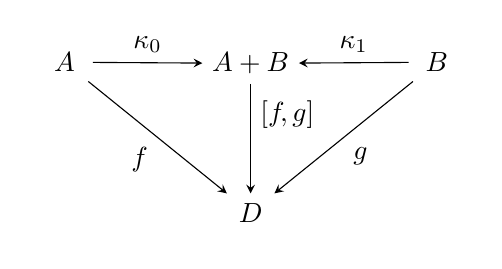
\begin{tikzpicture}[scale=1.2]
\matrix (m) [matrix of math nodes,row sep=4em,column sep=4em,minimum width=2em]
  {
     A & A + B & B \\
     {} & D & {} \\
  };
  \path[-stealth]
    (m-1-1) edge node [below left] {$f$} (m-2-2)
            edge node [above] {$\kappa_0$} (m-1-2)
    (m-1-2) edge node [above right] {$[f\!,g]$} (m-2-2)
    (m-1-3) edge node [above] {$\kappa_1$} (m-1-2)
            edge node [below right] {$g$} (m-2-2)
    ;
\end{tikzpicture}
\end{center}
\caption{The usual coproduct diagram} \label{figCoproductDiagram}
\end{figure}


\begin{definition}
A \emph{bifunctor} is a functor with two arguments. Formally, $F : \bbC \times \bbD \arr
\bbE$ is a bifunctor iff it is functorial in $\bbC$ and $\bbD$ separately, that
is for all fixed $C \in \bbC$ and $D \in \bbD$, both $F_C(D) = F(C \times D) : \bbD
\arr \bbE$ and $F_D(C) = F(C \times D) : \bbC \arr \bbE$ must be functors.
Furthermore, for arrows $f : C \arr C'$ in $\bbC$ and $g : D \arr D'$ in $\bbD$,
we must have $F_{D'}(f) \circ F_C(g) = F_{C'}(g) \circ F_D(f) : F(C \times D)
\arr F(C' \times D')$, where
\begin{IEEEeqnarray*}{rCl}
F_D(f : C \arr C') & = & F(f \times 1_D) : F(C \times D) \arr F(C' \times D) \\
F_C(g : D \arr D') & = & F(1_C \times g) : F(C \times D) \arr F(C \times D')
\end{IEEEeqnarray*}
\end{definition}

\begin{proposition}

For a fixed $D$, the object mapping $L_D : A \mapsto A \oplus D$ extends to a
functor.  Symmetrically for $R_D : A \mapsto D \oplus A$, and we have for all $f
: A \arr A'$ and $g : B \arr B'$, $L_{B'}(f) \circ R_A(g) = R_{A'}(g) \circ
L_B(f) : A \oplus B \arr A' \oplus B'$.  Therefore $\oplus : \text{Cppo} \times
\text{Cppo} \arr \text{Cppo}$ is a bifunctor. \qed

\end{proposition}

So while the separated sum is not the categorical coproduct, it is still a
useful construction and we can work with it as long as we keep in mind that
$[f\!,g]$ doesn't have the universal mapping property.

This sets up the stage for our following considerations.

\section{Fixpoint Semantics for Recursive Functions}
\label{secFixpointSemantics}

Using the constructions seen so far, we can show that certain recursive
functions are well-defined. This is the central idea of Scott's fixpoint
semantics for recursive programs, but it can also be employed for mathematical
purposes that don't concern programming.

First, we look at the factorial function, as it is a simple example that nicely
demonstrates the technique at work.

\todo{cite critique 1 in Arbib and Manes for the factorial example}

\begin{lemma} \label{lemPartialFunctionSpaceCppo}

Let $A, B$ be sets. The set of partial functions from $A$ to $B$, denoted
$[A \pfun B]$, is a cppo.

\end{lemma}

\begin{proof}

Let $f, g : A \pfun B$. Define $f \below g$ iff $f \subseteq g$, where we
consider $f$ and $g$ as their underlying graphs.

The totally undefined function $\emptyset = \bot$ is an element of $[A \pfun B]$
and satisfies $\bot \below g$ for all $g$.

If $F$ is a chain of functions, consider $\bigcup F$, the union of the graphs of
all functions in $F$. We have: if $f \in F$ then $f \subseteq \bigcup F$, so $f
\below \bigcup F$.  In other words $\bigcup F$ is an upper bound of $F$.

Furthermore if $g$ is an upper bound of $F$ then $\forall f \in F \ldotp f
\below g$, so $\bigcup F \below g$. In other words $\bigcup F$ is the lub of $F$
and it is justified to write $\lub F$

\end{proof}


The definition of $f \below g$ is equivalent to the following formula, which is
less easy to read, but lends itself better to proofs.
\begin{equation*}
\forall n \in \bbN \ldotp f(n)\isdefined \implies g(n)\isdefined\
\wedge\ f(n) = g(n)
\end{equation*}
Where $f(n)\isdefined$ is to be read as ``$f$ is defined at $n$''.

The following two lemmas are always useful for proving continuity.

\begin{lemma} \label{lemMonotoneAlwaysBelowLub}
Let $A, B$ be cpos, $f : A \arr B$ be a monotone function, and $C \subseteq A$
be a chain in A. Then $\lub f(C) \below f(\lub C)$.
\end{lemma}

\begin{proof}
We have:
\begin{IEEEeqnarray*}{rCl}
           && \forall a \in C \ldotp a \below \lub C \\
 & \implies & \forall a \in C \ldotp f(a) \below f(\lub C) \\
 & \implies & f(\lub C) \text{ is an upper bound of } f(C) \\
 & \implies & \lub f(C) \below f(\lub C)
\end{IEEEeqnarray*}
\end{proof}


\begin{lemma} \label{lemMonotoneIsContinuousFinite}
Let $A, B$ be cpos, $f : A \arr B$ be a monotone function, and $C \subseteq A$
be a finite chain in $A$. Then $f(\lub C) = \lub f(C)$.
\end{lemma}

\begin{proof}
We have $\lub C \in C$, because $C$ is finite. Therefore $f(\lub C) \in f(C)$,
and thus $f(\lub C) \below \lub f(C)$. Lemma \ref{lemMonotoneAlwaysBelowLub}
gives the converse direction.
\end{proof}




\begin{proposition} \label{propFactorialExists}

There exists a function $f : \bbN \arr \bbN$ such that
\begin{IEEEeqnarray}{rCl}
f(0) & = & 1 \label{eqnFactorial1} \\
f(n) & = & n \cdot f(n - 1) \quad\text{if}\ \ n > 0 \label{eqnFactorial2}
\end{IEEEeqnarray}

\end{proposition}

Proposition \ref{propFactorialExists} can be rephrased in different ways: the
recursive definition of the factorial function is not vacuous; it is not a
circular definition; it does not lead to infinite regress.

\todo{
That's interesting. In our case (see far below) we have at some point
$\pi(\_^\omega) = \pi(\kappa_1(\_^\omega)) = \pi(\_^\omega)$, a genuine circle
in the definition.  Yet we argue that the definition is not vacuous. What to
make of that? We surely have $\pi(\_^\omega)\!\uparrow$, $\pi(\_^\omega) = \bot$
so that's the ejection seat.
}

\begin{proof}
From \ref{lemPartialFunctionSpaceCppo} we know that $[\bbN \pfun
\bbN]$ is a cppo. Consider the function

\begin{equation*}
\varphi(g) = n \mapsto \left\{
  \begin{array}{lcl}
   1          & \text{if} & n = 0 \\
   n \cdot g(n-1) & \text{if} & n > 0
  \end{array}
\right.
\end{equation*}

$\varphi$ is not defined recursively, so it certainly is a function $[\bbN
\pfun \bbN] \arr [\bbN \pfun \bbN]$. If we can show that
$\varphi$ is continuous, then it is an arrow in Cppo, so by theorem
\ref{thmFixpoint} it has a fixpoint $f$ such that
\begin{IEEEeqnarray}{rCl}
f = \varphi(f) \label{eqnFactorialFixpoint}
\end{IEEEeqnarray}

Using equation (\ref{eqnFactorialFixpoint}) we proceed to show that the required
equations (\ref{eqnFactorial1}) and (\ref{eqnFactorial2}) hold.
\begin{IEEEeqnarray*}{rCl}
f(0) & = & \varphi(f)(0) = 1 \\
f(n) & = & \varphi(f)(n) = n \cdot f(n - 1) \quad\text{if}\ \ n > 0
\end{IEEEeqnarray*}

We still need to show that $\varphi$ is continuous. For that matter, first
observe that $\varphi$ is monotone: assume $f \below g$. To prove: $\varphi(f)
\below \varphi(g)$, i.e.
\begin{equation*}
\forall n \in \bbN \ldotp \varphi(f)(n)\isdefined \implies
\varphi(g)(n)\isdefined\ \wedge\ \varphi(f)(n) = \varphi(g)(n)
\end{equation*}
Let $n \in \bbN$.  Assume that
$\varphi(f)(n)\isdefined$.

If $n = 0$ then $\varphi(f)(n) = 1 = \varphi(g)(n)$.

If $n > 0$ then $\varphi(f)(n) = n \cdot
f(n - 1)$. As $\varphi(f)(n)\isdefined$, we must have
$f(n-1)\isdefined$, which by assumption implies $g(n-1)\isdefined \wedge\
f(n-1) = g(n-1)$, and thus $n \cdot f(n-1) = n \cdot g(n-1) = \varphi(g)(n)$.

In both cases, $\varphi(g)(n)\isdefined \wedge\ \varphi(f)(n) = \varphi(g)(n)$,
so $\varphi(f) \below \varphi(g)$, which proves that $\varphi$ is monotone.

It remains to show that $\varphi$ preserves lubs. Let $C$ be a chain in
$[\bbN \pfun \bbN]$. Then, because $\varphi$ is monotone,
$\varphi(C)$ is a chain as well, and both have lubs $\lub C$, $\lub \varphi(C)$.
To prove: $\varphi(\lub C) = \lub \varphi(C)$. It suffices to show inequality
$\below$ in both directions.

$\lub \varphi(C) \below \varphi(\lub C)$: By lemma
\ref{lemMonotoneAlwaysBelowLub}.

$\varphi(\lub C) \below \lub \varphi(C)$: For this direction, we have to delve
into $\varphi$. It suffices to show
\begin{equation*}
  \forall n \in \bbN \ldotp \varphi(\lub C)(n)\isdefined \implies
  (\lub \varphi(C))(n)\isdefined\ \wedge\ \varphi(\lub C)(n) = (\lub
  \varphi(C))(n)
\end{equation*}
Let $n \in \bbN$. Assume $\varphi(\lub C)(n)\isdefined$.

If $n = 0$ then $\varphi(\lub C)(0) = 1$, and we have $\forall f \in C
\ldotp \varphi(f)(0) = 1$, so $(\lub \varphi(C))(0)~= 1$.

If $n > 0$ then $\varphi(\lub C)(n) = n \cdot (\lub C)(n - 1)$, and thus from
$\varphi(\lub C)(n)\isdefined$ we get $(\lub C)(n - 1)\isdefined$. But then
there must be a $g$ in $C$ such that $g(n-1)\isdefined$ and $g(n-1) = (\lub C)(n
- 1)$. But then $n \cdot g(n-1)\isdefined$, therefore $\varphi(g)(n)\isdefined$,
which implies $(\lub \varphi(C))(n)\isdefined$ and we have:
\begin{IEEEeqnarray*}{c}
(\lub \varphi(C))(n) = \varphi(g)(n) = n \cdot g(n-1) = n \cdot (\lub C)(n-1)
 = \varphi(\lub C)(n)
\end{IEEEeqnarray*}

\end{proof}


The strategy just employed is prototypical for proving the existence of a
recursively defined function $f$. First, find a non-recursive higher-order
function corresponding to $f$ in spirit of our $\varphi$. Then prove $\varphi$
to be continuous and show that its fixpoint fulfills the desired definition.


\section{$1+X$ and $1+X+X$}

\todo{explain what $1+X$, $1+X+X$ are (simultaneous separated sum!) and why we
want all that follows.}

\begin{lemma} \label{lemLambek}
todo Lambek's lemma op: final coalgebras are isomorphisms.
\end{lemma}

\subsection{Draft: Naming}

The things involved need names.

Base functors:
\begin{IEEEeqnarray*}{rCl}
F(X) & = & 1 + X \\
G(X) & = & 1 + X + X
\end{IEEEeqnarray*}

Their final coalgebras:
\begin{IEEEeqnarray*}{rCl}
\nu F & = & \alpha : A \leftrightarrow FA \\
\nu G & = & \beta : B \leftrightarrow GB
\end{IEEEeqnarray*}



\begin{proposition} \label{propEpsilonPiExist}
There exists a continuous embedding-projection pair
\begin{IEEEeqnarray*}{RCCl}
\varepsilon : & A & \arr & B \\
\pi         : & B & \arr & A
\end{IEEEeqnarray*}
such that $\pi \circ \varepsilon = \text{id}_A$.
\end{proposition}


\todo{define $f \below g$ for $f, g : [A \arr B]$ and lub of chains pointwise}


Greatest fixpoints of functors arise as limits of left chains. See theorem
11.3.14 in \cite{Manes1986}.  \begin{IEEEeqnarray*}{c}
\cdots\ \arr\ F^3(1)\ \arr\ F^2(1)\ \arr\ F(1)\ \arr\ 1
\end{IEEEeqnarray*}
Intuitively, the cppos we use for data structure semantics arise by
$\omega$-fold iteration of the base functor on the terminal object $1$. The
first few iterations for the functor $F(X) = 1 + X$, together with the partial
order induced by the separated sum, are illustrated in figure
\ref{figFirstIterationsOfF}. In each iteration, the cppo of the previous step is
lifted through $\kappa_1$ to the upper right, and fresh $\kappa_0(\bot)$ and
$\bot$ are introduced.


\begin{figure}
\begin{center}
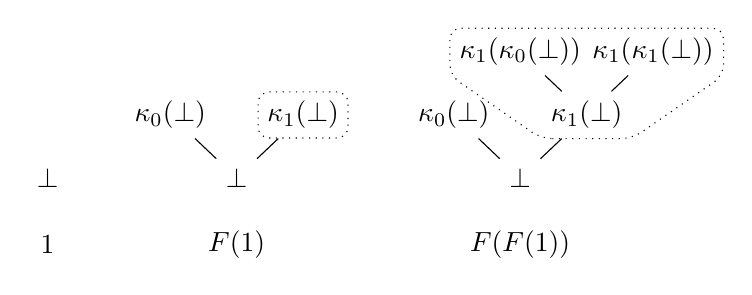
\begin{tikzpicture}[scale=1.2]
  \node {$\bot$} [grow'=up, sibling distance=4.0em, level distance=1.9em]
  ;

  \node at (0,-0.7) {$1$};

  \node at (2,0) {$\bot$} [grow'=up, sibling distance=4.0em, level distance=1.9em]
    child { node {$\kappa_0(\bot)$} }
    child { node [draw,dotted,rounded corners] {$\kappa_1(\bot)$} }
  ;

  \node at (2,-0.7) {$F(1)$};

  \node at (5,0) {$\bot$} [grow'=up, sibling distance=4.0em, level distance=1.9em]
    child { node {$\kappa_0(\bot)$} }
    child {
      node [name=foo] { $\kappa_1(\bot)$ }
      child { node [name=bar] { $\kappa_1(\kappa_0(\bot))$ } }
      child { node [name=baz] { $\kappa_1(\kappa_1(\bot))$ } }
    }
  ;

  \node at (5,-0.7) {$F(F(1))$};

  \path [draw,dotted,rounded corners] (foo.south west) -- (foo.south east)
    -- (baz.south east)
    -- (baz.north east)
    -- (bar.north west)
    -- (bar.south west)
    -- cycle
  ;

\end{tikzpicture}
\end{center}
\caption{The first iterations of $1+X$ on $1$. Marked parts indicate the
inclusion of the previous iteration.}
\label{figFirstIterationsOfF}
\end{figure}

The final coalgebras $A$ and $B$, together with their ordering are depicted in
the Hasse diagrams of figures \ref{figDomainOfLazyNaturals} and
\ref{figDomainOfNuF}. These figures employ some notational simplification.

\begin{figure}[th]
\begin{center}
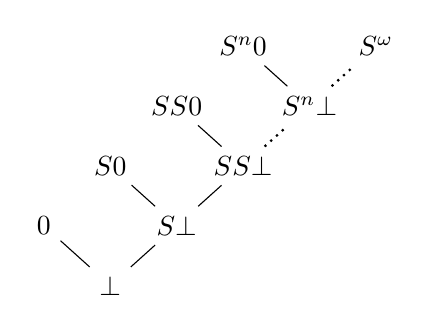
\begin{tikzpicture}[scale=1.2]
  \node {$\bot$} [grow'=up, sibling distance=4.0em, level distance=1.8em]
    child { node {$0$} }
    child
    {
      node {$S\bot$}
      child { node {$S0$} }
      child
      {
        node {$SS\bot$}
        child { node {$SS0$} }
        child [thick, dotted]
        {
          node {$S^n\bot$}
          child [thin, solid] { node {$S^n0$} }
          child { node {$S^\omega$} }
        }
      }
    }
  ;
\end{tikzpicture}
\end{center}
\caption{The cppo $(A, \below)$.}
\label{figDomainOfLazyNaturals}
\end{figure}

\begin{figure}[th]
\begin{center}
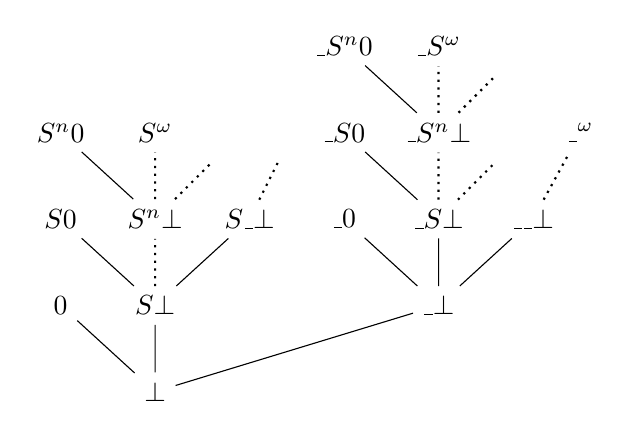
\begin{tikzpicture}
 [ grow'=up
 , scale=1.2
 , level distance=2.6em
 , level 1/.style={sibling distance=3cm}
 , level 2/.style={sibling distance=1cm}
 , normal/.style={thin, solid}
 , skipping/.style={thick, dotted}
 , and so on/.style={thick, dotted, sibling distance=0.6cm, level distance=0.6cm}
 ]
  \node {$\bot$}
    child [sibling distance=1cm] { node {$0$} }
    child
    {
      node {$S\bot$}
      child { node {$S0$} }
      child [skipping]
      {
        %node {$SS\bot$}
        %child { node {$SS0$} }
        %child [skipping]
        %{
          node {$S^n\bot$}
          child [normal] { node {$S^n0$} }
          child [skipping] { node {$S^\omega$} }
          child [and so on] {}
        %}
        %child [and so on] {}
      }
      child
      {
        node {$S\_\bot$}
        child [missing] {}
        child [and so on] {}
      }
    }
    child
    {
      node {$\_ \bot$}
      child { node {$\_0$} }
      child
      {
        node {$\_S\bot$}
        child { node {$\_S0$} }
        child [skipping]
        {
          node {$\_S^n\bot$}
          child [normal] { node {$\_S^n0$} }
          child { node {$\_S^\omega$} }
          child [and so on] {}
        }
        child [and so on] {}
      }
      child
      {
        node {$\_\_\bot$}
        child [missing] {}
        %child [missing] {}
        child [skipping] { node {$\_^\omega$} }
      }
    }
  ;
\end{tikzpicture}
\end{center}
\caption{The cppo $(B, \below)$.}
\label{figDomainOfNuF}
\end{figure}

\begin{lemma} \label{lemEpsilonExists}
There is a function $\varepsilon : A \arr B$ such that

\begin{equation*}
\varepsilon(a) = \left\{
  \begin{array}{rcl}
   \bot_B & \text{if} & a = \bot_A \\
   \beta^{-1}(\kappa_0(a')) & \text{if} & \beta(a) = \kappa_0(a') \\
   \beta^{-1}(\kappa_1(\varepsilon(a'))) & \text{if} & \beta(a) = \kappa_1(a')
  \end{array}
\right.
\end{equation*}

\end{lemma}

This specification is highly technical, and it's hard to see that there really
is not much going on.  From now on we employ some notational simplifications to
make matters more clear.

First, lemma \ref{lemLambek} allows us to be liberal with $\alpha$ and $\beta$,
so we leave them out and view an element of $A$ as also being of $1 + A$ and
vice versa. Same for $B$ and $1+B+B$. When appropriate, we write ``$x$ is of the
form $S(-)$'' instead of $\exists x' \ldotp \alpha(x) = S(x')$ .

Second, $1$ as the terminal object in Cppo is a one-element set, so
$\kappa_0(a')$ can be of only one form, for which we write $0$.

Third, we write $S$ for $\kappa_1$ and $\_$ for $\kappa_2$.

The requirements for \ref{lemEpsilonExists} then become:

\begin{equation*}
\varepsilon(a) = \left\{
  \begin{array}{rcl}
   \bot & \text{if} & a = \bot \\
   0 & \text{if} & a = 0 \\
   S(\varepsilon(a')) & \text{if} & a = S(a')
  \end{array}
\right.
\end{equation*}

From this it is easier to see that $\varepsilon$ doesn't do anything except
replacing the constructors of $1+A$ by their equivalent of $1+B+B$. The proof
proceeds similarly to the one of \ref{propFactorialExists}, but now we have
slightly more work to do. We need the following lemmas.


\begin{lemma} \label{lemDefinitionBelowAandB}
For $x,y \in A$, we have $x \below y$ iff
\begin{IEEEeqnarray*}{rtl}
& & x = \bot \\
& or\quad & x = y \\
& or\quad & x = S(x') \aand y = S(y') \aand x' \below y'
\end{IEEEeqnarray*}

For $x,y \in B$, we have $x \below y$ iff
\begin{IEEEeqnarray*}{tlClClCl}
& x = \bot \\
or\quad & x = y \\
or\quad & x = S(x') & \aand & y & = & S(y') & \aand & x' \below y' \\
or\quad & x = \_(x') & \aand & y & = & \_(y') & \aand & x' \below y'
\end{IEEEeqnarray*}
\qed
\end{lemma}


\begin{lemma} \label{lemCoFiniteSubsetLub}

If $C$ is an infinite chain and $C' \subseteq C$ a co-finite subset, then $\lub
C = \lub C'$. \qed

\end{lemma}


\begin{lemma} \label{lemChainInversion}

If $C$ is an infinite chain in $A$ such that $\lub C = S(a)$ for some $a \in A$,
then
\begin{enumerate}

  \item \label{lemChainInversion1} all but finitely many $x \in C$ are of the
  form $S(-)$.  In other words, there is a co-finite subset $C'$ of $C$ having
  the same lub, where all elements of $C'$ are of the form $S(-)$.

  \item \label{lemChainInversion2} The set $C'' = \set{x' \mid S(x') \in C'}$ is
  a chain, and $\lub C = S(\lub C'')$.
\end{enumerate}

\end{lemma}

Intuitively, this lemma states that if
\begin{IEEEeqnarray*}{c}
\bot \below S(x_0) \below S(x_1) \below S(x_2) \below \ldots
\end{IEEEeqnarray*}
is a chain, then so is
\begin{IEEEeqnarray*}{c}
x_0 \below x_1 \below x_2 \below \ldots
\end{IEEEeqnarray*}
and the lub of the first is the same as the successor of the lub of the second.
This lemma is the opposite of lemma \ref{lemMonotoneAlwaysBelowLub}, the latter
holding for any cpo and monotone function, while here the interaction between
$S$ and $\below$ is required.


\begin{proof}

(Lemma \ref{lemChainInversion}) \ref{lemChainInversion1}. Let $C$ be an infinite
chain such that $\lub C = S(a)$, and assume towards a contradiction that
infinitely many elements are not of the form $S(-)$. Then, for each $x \in C$,
there is a $y \in C$ such that $x \below y \below S(a)$ and $y$ is not of
the form $S(-)$. Then, by definition of $\below$, $y$ must be $\bot$. But
then $\bot$ is an upper bound of $C$, which contradicts the assumption that
$S(a)$ is the least upper bound of $C$.

\ref{lemChainInversion2}. We show that the order on $C''$ is total. Let $x', y'
\in C''$. Then by definition of $C''$, there are $x, y \in C'$ such that $x
\below y \aand x = S(x') \aand y = S(y')$. By definition of $\below$ this gives
$x' \below y'$.

It remains to show that $\lub C = S(\lub C'')$. It suffices to show that $a =
\lub C''$, because then $\lub C = S(a) = S(\lub C'')$. We calculate:
\begin{IEEEeqnarray*}{rCls}
&& \forall x' \in C'' \ldotp S(x') \below S(a) & ($S(a)$ upper bound of $C'$) \\
& \implies & \forall x' \in C'' \ldotp x' \below a & (definition $\below$)\\
& \implies & a \text{ is an upper bound of } C''.
\end{IEEEeqnarray*}

Let $b$ be an upper bound of $C''$. Then
\begin{IEEEeqnarray*}{rCls}
&& \forall x' \in C'' \ldotp x' \below b \\
& \implies & \forall x' \in C'' \ldotp S(x') \below S(b) & ($S$ monotone)\\
& \implies & S(b) \text{ is an upper bound of } C' & (definition $C''$) \\
& \implies & \lub C' = S(a) \below S(b) & (S(a) least upper bound) \\
& \implies & a \below b & (definition $\below$) \\
& \implies & a \text{ is the least upper bound of } C''.
\end{IEEEeqnarray*}

\end{proof}


\begin{proof}

(Lemma \ref{lemEpsilonExists}) Define $\varphi : [A \arr B] \arr [A \arr B]$ as:

\begin{equation*}
\varphi(f) = a \mapsto \left\{
  \begin{array}{rcl}
   \bot & \text{if} & a = \bot \\
   0 & \text{if} & a = 0 \\
   S(f(a')) & \text{if} & a = S(a')
  \end{array}
\right.
\end{equation*}

As we now work in Cppo, $[A \arr B]$ denotes the set of continuous functions
from $A$ to $B$. To prove:
\begin{enumerate}[noitemsep]
\item \label{proofEpsilonExists1} $\varphi$ maps continuous functions to
continuous functions.
\item \label{proofEpsilonExists2} $\varphi$ is itself continuous.
\item \label{proofEpsilonExists3} $\varepsilon$ as the fixpoint of $\varphi$
satisfies the desired equation.
\end{enumerate}

\ref{proofEpsilonExists1}. Let $f : A \arr B$ be continuous. We have to show
that $\varphi(f)$ is monotone and preserves lubs.

Monotonicity: let $x, y \in A$ such that $x \below y$.

If $x = \bot$ then $\varphi(f)(x) = \bot \below \varphi(f)(y)$ always.

If $x = 0$ then $y = 0$ as well, so $\varphi(f)(x) = \varphi(f)(y)$.

If $x = S(x')$ then, because $x \below y$, there must be a $y'$ such that $y =
S(y')$ and $x' \below y'$. But $S$ and $f$ are both monotone, so
\begin{equation*}
\varphi(f)(x) = S(f(x')) \below S(f(y')) = \varphi(f)(y).
\end{equation*}

Lub preservation: Let $C$ be a chain in $A$. To prove: $\varphi(f)(\lub C) =
\lub \varphi(f)(C)$.

If $\lub C = \bot$ then $C$ is finite, and the conclusion follows by lemma
\ref{lemMonotoneIsContinuousFinite}.

If $\lub C = 0$ then again $C$ must be finite.

If $\lub C = S(a)$ for some $a \in A$ then if $C$ is finite, we're done. Let $C$
be infinite. Then, using lemma \ref{lemChainInversion} and its constructions
$C'$ and $C''$, we calculate:
\begin{IEEEeqnarray*}{rCl's}
&& \varphi(f)(\lub C) \\
& = & \varphi(f)(S(a)) \\
& = & S(f(a)) & (definition $\varphi$) \\
& = & S(f(\lub C'')) & (lemma \ref{lemChainInversion}) \\
& = & \lub S(f(C'')) & ($S, f$ continuous) \\
& = & \lub \varphi(f)(S(C'')) & (definition $\varphi$) \\
& = & \lub \varphi(f)(C') & (definition $C'$) \\
& = & \lub \varphi(f)(C) & (lemma \ref{lemCoFiniteSubsetLub})
\end{IEEEeqnarray*}

\ref{proofEpsilonExists2}. Monotonicity: Let $f,g \in [A \arr B]$ such that $f
\below g$.  To prove: $\varphi(f) \below \varphi(g)$, i.e. $\forall a \in A
\ldotp \varphi(f)(a) \below \varphi(g)(a)$.  The cases $a = \bot$ and $a = 0$
are trivial, so let $a = S(a')$. Then
\begin{IEEEeqnarray*}{c}
\varphi(f)(a) = S(f(a')) \below S(g(a')) = \varphi(g)(a).
\end{IEEEeqnarray*}

Lub preservation: Let $C = \set{f_n \mid n \in \bbN}$ be a chain
in $[A \arr B]$.  To prove: $\varphi(\lub C) = \lub \varphi(C)$. Let $a \in
A$. Because lubs of function chains are defined pointwise, it suffices to show
$\lub \varphi(C)(a) = \varphi(\lub C)(a)$.

If $a = \bot$ then $\varphi(f)(a) = \bot$ for all $f \in C$, so
\begin{IEEEeqnarray*}{c}
    \lub \varphi(C)(a)
  = \lub \set{\bot}
  = \bot
  = \varphi(\lub C)(a).
\end{IEEEeqnarray*}

If $a = 0$ then $\varphi(f)(a) = 0$ for all $f \in C$, so
\begin{IEEEeqnarray*}{c}
    \lub(\varphi(C)(a))
  = \lub \set{0}
  = 0
  = \varphi(\lub C)(0).
\end{IEEEeqnarray*}

If $a = S(a')$ then
\begin{IEEEeqnarray*}{rClu}
     && \lub(\varphi(C)(a)) \\
  & = & \lub \set{S(f_n(a')) \mid n \in \bbN} & (definition of $\varphi$) \\
  & = & S(\lub \set{f_n(a') \mid n \in \bbN}) & (S is continuous) \\
  & = & S((\lub C)(a')) & (lubs are defined pointwise) \\
  & = & \varphi(\lub C)(a) & (definition of $\varphi$)
\end{IEEEeqnarray*}

Now we know that $\varphi$ is continuous, so we use the fixpoint theorem to
conclude that $\varphi$ has a least fixpoint, call it $\varepsilon$. It remains
to show that $\varepsilon$ has the desired properties.

\ref{proofEpsilonExists3}. We have $\varepsilon = \varphi(\varepsilon)$. Let $a
\in A$.

If $a = \bot$ then $\varepsilon(a) = \varphi(\varepsilon)(a) = \bot$.

If $a = 0$ then $\varepsilon(a) = \varphi(\varepsilon)(a) = 0$.

If $a = S(a')$ then $\varepsilon(a) = \varphi(\varepsilon)(a) =
S(\varepsilon(a'))$.

\end{proof}

The proof that $\pi$ exists and has the desired properties follows the same
sche\-ma as above, except we have one more case to consider. We leave out all the
boilerplate and concentrate on the interesting cases.

\begin{lemma} \label{lemPiExists}
There is a function $\pi : B \arr A$ such that

\begin{IEEEeqnarray*}{c}
\pi(b) = \left\{
  \begin{array}{rcl}
   \bot_A & \text{if} & b = \bot_B \\
   0_A & \text{if} & b = 0_B \\
   S_A(\pi(b')) & \text{if} & b = S_B(b') \\
   \pi(b') & \text{if} & b = \_(b')
  \end{array}
\right.
\end{IEEEeqnarray*}

\end{lemma}

\begin{proof}
(Lemma \ref{lemPiExists}) Define $\psi : [B \arr A] \arr [B \arr A]$ as:

\begin{IEEEeqnarray*}{c}
\psi(f) = b \mapsto \left\{
  \begin{array}{rcl}
   \bot & \text{if} & b = \bot \\
   0 & \text{if} & b = 0 \\
   S(f(b')) & \text{if} & b = S(b') \\
   f(b') & \text{if} & b = \_(b')
  \end{array}
\right.
\end{IEEEeqnarray*}

To prove:
\begin{enumerate}[noitemsep]
\item \label{proofPiExists1} $\psi$ maps continuous functions to
continuous functions.
\item \label{proofPiExists2} $\psi$ is itself continuous.
\item \label{proofPiExists3} $\pi$ as the fixpoint of $\psi$
satisfies the desired equation.
\end{enumerate}

\ref{proofPiExists1}. Let $f \in [B \arr A]$. To prove: $\psi(f)$ is continuous.

Monotonicity: Let $x,y \in B$ such that $x \below y$.

If $x = S(x')$ then by lemma \ref{lemDefinitionBelowAandB} there must be a $y'$
such that $y = S(y')$ and $x' \below y'$. We have:
\begin{IEEEeqnarray*}{c}
\psi(f)(x) = S(f(x')) \below S(f(y')) = \psi(f)(y).
\end{IEEEeqnarray*}

If $x = \_(x')$ then there must be a $y'$ such that $y = \_(y')$ and $x' \below
y'$. We have:
\begin{IEEEeqnarray*}{c}
\psi(f)(x) = f(x') \below f(y') = \psi(f)(y).
\end{IEEEeqnarray*}


Lub preservation: Let $C$ be a chain in $B$. To prove: $\psi(f)(\lub
C) = \lub \psi(f)(C)$.

\todo{we need a chain inversion lemma similar to \ref{lemChainInversion}}

If $C$ is infinite and $\lub C = S(b)$ for some $b \in B$, then:
\begin{IEEEeqnarray*}{rCl's}
&&    \psi(f)(\lub C) \\
& = & \psi(f)(S(b)) \\
& = & S(f(b)) \\
& = & S(f(\lub C'')) & (todo chain inversion lemma) \\
& = & \lub S(f(C'')) \\
& = & \lub \psi(f)(S(C'')) \\
& = & \lub \psi(f)(C') \\
& = & \lub \psi(f)(C)
\end{IEEEeqnarray*}

If $C$ is infinite and $\lub C = \_(b)$ for some $b \in B$, then:
\begin{IEEEeqnarray*}{rCl's}
&&    \psi(f)(\lub C) \\
& = & \psi(f)(\_(b)) \\
& = & f(b) \\
& = & f(\lub C'') & (todo chain inversion lemma) \\
& = & \lub f(C'') \\
& = & \lub \psi(f)(\_(C'')) \\
& = & \lub \psi(f)(C') \\
& = & \lub \psi(f)(C)
\end{IEEEeqnarray*}

\ref{proofPiExists2}. Monotonicity: Let $f, g \in [B \arr A]$ such that $f
\below g$. To prove: $\psi(f) \below \psi(g)$, which is equivalent to $\forall b
\in B \ldotp \psi(f)(b) \below \psi(g)(b)$. Let $b \in B$.

If $b = S(b')$ then
\begin{IEEEeqnarray*}{c}
\psi(f)(b) = S(f(b')) \below S(g(b')) = \psi(g)(b).
\end{IEEEeqnarray*}

If $b = \_(b')$ then
\begin{IEEEeqnarray*}{c}
\psi(f)(b) = f(b') \below g(b') = \psi(g)(b).
\end{IEEEeqnarray*}

Lub preservation: Let $C$ be a chain in $[B \arr A]$. To prove: $\psi(\lub C) =
\lub \psi(C)$. Lubs of function chains are defined pointwise, so it suffices to
show that $\forall b \in B \ldotp \psi(\lub C)(b) = \lub(\psi(C)(b))$. Let $b
\in B$.

If $b = S(b')$ then
\begin{IEEEeqnarray*}{rClu}
     && \lub(\psi(C)(b)) \\
  & = & \lub \set{S(f_n(b')) \mid n \in \bbN} & (definition of $\psi$) \\
  & = & S(\lub \set{f_n(b') \mid n \in \bbN}) & (S is continuous) \\
  & = & S((\lub C)(b')) & (lubs are defined pointwise) \\
  & = & \psi(\lub C)(b) & (definition of $\psi$)
\end{IEEEeqnarray*}

If $b = \_(b')$ then
\begin{IEEEeqnarray*}{rClu}
     && \lub(\psi(C)(b)) \\
  & = & \lub \set{f_n(b') \mid n \in \bbN} & (definition of $\psi$) \\
  & = & (\lub C)(b') & (lubs are defined pointwise) \\
  & = & \psi(\lub C)(b) & (definition of $\psi$)
\end{IEEEeqnarray*}

By the fixpoint theorem, $\psi$ has a least fixpoint $\pi$. We have $\pi =
\psi(\pi)$, and we still need to prove the equation of the lemma.

\ref{proofPiExists3}. Let $b \in B$.

If $b = \bot$ then $\pi(b) = \psi(\pi)(b) = \bot$.

If $b = 0$ then $\pi(b) = \psi(\pi)(b) = 0$.

If $b = S(b')$ then $\pi(b) = \psi(\pi)(b) = S(\pi(b'))$.

If $b = \_(b')$ then $\pi(b) = \psi(\pi)(b) = \pi(b')$.

\end{proof}

We are now ready to conclude the result of this section.

\begin{proof}
(Proposition \ref{propEpsilonPiExist}) The existence of $\varepsilon$ and $\pi$
was proven in lemmas \ref{lemEpsilonExists} and \ref{lemPiExists}. To show that
this is an embedding-projection-pair, i.e. $\pi \circ \varepsilon =
\text{id}_A$, let $a \in A$.

If $a = \bot$ then $\pi(\varepsilon(\bot)) = \pi(\bot) = \bot$.

If $a = 0$ then $\pi(\varepsilon(0)) = \pi(0) = 0$.

If $a = S(a')$ then $\pi(\varepsilon(S(a'))) = \pi(S(\varepsilon(a'))) =
S(\pi(\varepsilon(a')))$.

In all cases, $\alpha \circ (\pi \circ \varepsilon) = F(\pi \circ \varepsilon)
\circ \alpha$, which means that the following diagram commutes, and because
$\alpha$ is the final coalgebra of $F$, this implies $\pi \circ \varepsilon =
\text{id}_A$.
\begin{figure}[h]
\begin{center}
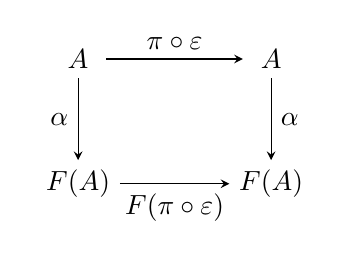
\begin{tikzpicture}
\matrix (m) [matrix of math nodes,row sep=3em,column sep=4em,minimum width=2em]
  {
     A & A \\
     F(A) & F(A) \\
  };
  \path[-stealth]
    (m-1-1) edge node [left] {$\alpha$} (m-2-1)
            edge node [above] {$\pi \circ \varepsilon$} (m-1-2)
    (m-2-1.east|-m-2-2) edge node [below] {$F(\pi \circ \varepsilon)$} (m-2-2)
    (m-1-2) edge node [right] {$\alpha$} (m-2-2);
\end{tikzpicture}
\end{center}
\end{figure}

\end{proof}

It would be nice to have, for the other direction, at least $\varepsilon \circ
\pi \below \text{id}_B$, but unfortunately that's not the case. To see why,
consider the counterexample
\begin{IEEEeqnarray*}{rCl}
\varepsilon(\pi(\_S0)) = \varepsilon(S0) = S0
\end{IEEEeqnarray*}
where $\_S0$ and $S0$ are not related by $\below$ in $B$.

%\section{Junkyard}

%\begin{figure}[ht]
%\begin{center}
%\begin{tikzpicture}
%\matrix (m) [matrix of math nodes,row sep=3em,column sep=4em,minimum width=2em]
  %{
     %A & B \\
     %C & D \\
  %};
  %\path[-stealth]
    %(m-1-1) edge node [left] {$f$} (m-2-1)
            %edge node [above] {$g$} (m-1-2)
    %(m-2-1.east|-m-2-2) edge node [below] {$h$} (m-2-2)
    %(m-1-2) edge node [right] {$e$} (m-2-2);
%\end{tikzpicture}
%\end{center}
%\caption{Example of a commutative diagram}
%\end{figure}


%\section{Further directions}

\section{Bibliographic notes}

This work is based on chapter 7 of the PhD thesis of Venanzio Capretta
\cite{Capretta2002}, where coinductive natural numbers are discussed.  Some
treatment of lazy natural numbers can be found in \cite{Escardo1993}.

A short introduction to denotational semantics can be found in
\cite{Allison1986}, while \cite{Gunter1992} is a more comprehensive treatment of
that topic.  A view on domain theory and denotational semantics from the
perspective of category theory can be found in \cite{Pierce1991},
\cite{Bird1997}, \cite{Mitchell1996} and \cite{BarrWells1990}.


\bibliographystyle{plain}
\bibliography{computer_science}
\end{document}

% vim: textwidth=80:spell:spelllang=en_us
